\documentclass[10pt]{article}
\usepackage[top=0.75in, bottom=0.5in, left=0.5in, right=0.5in]{geometry}
\usepackage{amsmath,amsfonts, color, booktabs, centernot, textcomp,amssymb,graphicx,verbatim,enumerate, bbm}
%\usepackage [autostyle, english = american]{csquotes}
\usepackage [style = american]{csquotes}
\MakeOuterQuote{"}
\usepackage{algorithm} % Boxes/formatting around algorithms
\usepackage[noend]{algpseudocode} % Algorithms
\usepackage{wrapfig}
\usepackage{fancyhdr}
\pagestyle{fancy}
%\setlength\parindent{0pt}
\newcounter{problemnumber}
\def\Name{Leah Dickstein}  % Your name

\title{\vspace{-5ex} CSoI Personal Statement}
\author{\Name \vspace{-2ex}}
\date{}
\lhead{CSoI Personal Statement: \Name}


\begin{document}
\maketitle

% “While Shannon’s Theory of Information was originally applied to mathematics and electrical engineering, it is now applied in many other areas, including cryptography, neurobiology, language processing, and thermal physics.  Based on your knowledge of basic Information Theory, describe how it may be applied to a research project of your interest.”

%\subsection*{Introduction}

\subsection*{Personal Story}
When I entered university, I planned to study Chemical Biology. I had done a biology internship in high school, and I knew I loved research. I imagined myself pursuing a career in research, and Chemical Biology (I'm far too curious to be confined to a single subject) seemed the natural route to go. I had no idea what research in electrical engineering or math was like, and I didn't understand how research could be conducted without some kind of lab work.\\

The spring of my freshman year in university, my life changed. Following the recommendation of some friends, I took two courses for "fun": \textit{Introduction to Discrete Mathematics and Probability} and \textit{Introduction to Systems and Signals}. These courses introduced me to how math concepts were fundamental to technologies used everyday throughout the world. This subject, \textit{Math}, had been used to revolutionize the world, and its sister subject Electrical Engineering and Computer Science was touching and changing all industries. I didn't feel competent enough to push the boundaries of knowledge in math or theoretical EECS, but I definitely wanted to learn more and challenge myself.\\

I attended a talk given by graduate student Gireeja Ranade on her research. One topic stood out to me, so I read the paper Gireeja had written on it. I talked to Gireeja about her paper to understand it better, and in the process of understanding we agreed to work together on research the following summer. This was how I was introduced to information theory. I began working on this project the summer after freshman year of college. At the time, information theory was a mythical concept of using math to quantize "information", or how much we need to know to make decisions and interact with the world. Thankfully, information theory and math are no longer mythical, out-of-reach concepts to me. Thanks to my greater understanding, I am now captivated by the deep beauty within these subjects, and I would like to pursue these subjects further.\\

Since beginning the project, I have taken upper-division courses in probability and algorithms. This upcoming summer I will participate in Los Alamos Dynamics Summer School to further my studies in control theory and dynamics. In the fall I plan on taking courses in signals and abstract algebra, as well as TA-ing the freshman-year course \textit{Designing Information Devices and Systems}.
%\textcolor{red}{These courses and the teaching experience will develop me further.}

\subsection*{Research Interest}
% In many research papers dealing with communications and information theory, channels are treated as if they were instantaneous. Observations are sampled and controls are applied instantaneously, as the focus of the study is typically on the \textcolor{red}{control technique}. 
Shannon's 1948 paper "A Mathematical Theory of Communication" mentions delay, stating "Delay is generally required to approach the ideal encoding. It now has the additional function of allowing a large sample of noise to affect the signal before any judgment is made at the receiving point as to the original message." (p.25) Shannon theory requires delay (blocklength) to approach infinity to achieve channel capacity. This is not representative of real-world applications, where message transmission or control actions must take place within a finite time. In control systems the controller must take an action at a finite time based on the message it received, since a plant waiting for a control grows increasingly unstable. As an engineer, should I naively minimize or maximize the delay present in my control system? Will delay be good or bad for the system? The answer is not obvious. This is precisely the tradeoff we wish to explore and grasp.\\

%segway from Shannon to real-world applications have finite delay instead of infinite delay
%Shannon says we should use infinite delay but in real world we can't. For all real world systems, we need to eventually act. Who knows where the system is going?
%Maybe don't break up personal story and motivation

Waiting allows more bits of information to be observed and sent to the controller. This leads to more precise controls, which leads to greater controllability. In addition, having more bits available means we can allocate bits for parity, which increases message decoding probability. This in turn increases the controllability of the system. There is a tension present between control precision and message decoding probability, since with a fixed codeword length (fixed delay) allocating bits to parity decreases bits available for meaningful information. With larger delay, however, the control is given more flexibility in choosing the rate of transmission, such that we can approach the optimal encoding rate. \\

%(This is synonymous to Shannon claiming that we can achieve the capacity of a channel given infinite blocklength / encoding strategies, but in reality we are restricted to a finite blocklength regime.)

%The flipside to this is that every real-world system has a limit on the delay it can handle. We chose quantization noise because it is significantly impacted by delay, and can thus reflect effects from delay on the system.
It initially appears that we want the largest delay possible in our system. Most real-world systems need interaction or feedback from the controller to perform an action on the environment, meaning that we cannot allow infinite delay. We examine the instability that delay causes through quantization noise. As delay increases the effective system gain increases, because our system grows more before our control is applied. Given that we only have $m$ bits to quantize the state, the quantization noise will also increase. Thus, quantization noise \textit{grows worse} with time, which is something we would expect to see in a real-world system. It manifests in a multiplicative form, which was shown previously in work by Schenato et al.\footnote{S.Dey, A. Chiuso, L. Schenato. Remote estimation with noisy measurements subject to packet loss and quantization noise. \textit{Automatica} 2013} 

%If we wait too long or let delay grow too large, the noise will steadily increase to the point that we lose controllability.

\subsection*{Problem Setup and Initial Results}
Delay can both stabilize and destabilize a control system. This naturally leads to the question: how do we characterize the tradeoff? What is the optimal delay given certain system parameters? To model this, we use the following system:

\begin{minipage}{0.4\textwidth}
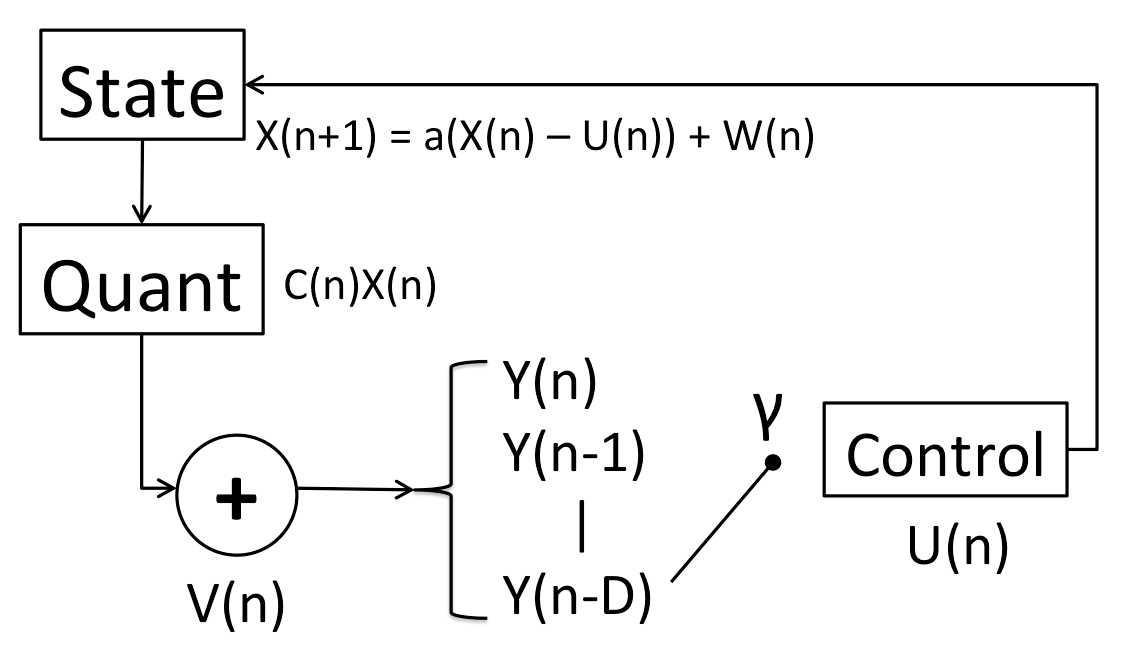
\includegraphics[width=0.7\textwidth]{sys_dynamics_2} 
\end{minipage}
\begin{minipage}{0.5\textwidth}
\[ X(n+1) = a(X(n) - U(n)) + W(n) \]
\[ Y(n) = \left\{
     \begin{array}{ll}
       Q(X(n)) + V(n) & : n \equiv 0 \text{ (mod D + 1)}\\
       0 & : \text{else}
     \end{array}
   \right. \]
\[ Q(X(n)) = C(n)X(n) \]
\[ U(n) = \left\{
     \begin{array}{ll}
       L[X(n) \; | \; Y(n-D)] & : n \equiv 0 \text{ (mod  D + 1)}\\
       0 & : \text{else}
     \end{array}
   \right. \]
\end{minipage}\\

Here, n is the time index, X is the scalar state of the system, Y is the observation, and U is the control. W $\sim N(0,\sigma^2_w)$ is system noise and V $\sim N(0, \sigma^2_v)$ is observation noise. $Q$ is the function for quantization. When we make an observation, we quantize the state of the system into $m$ bits. Here, using the formula from Rate Distortion Theory\footnote{Thomas Cover and Joy Thomas. Elements of Information Theory. 2006} we model quantization noise as a multiplicative noise $C(n) \sim N(1, 2^{-2m})$.\\

Given a delay $D$, where $D = 0$ represents instantaneous communication/transmission, we transmit the $m$ message bits as $D+1$ packets to the controller. Currently, encoding is represented by a Reed-Solomon code. We model the channel as a Ber($\frac{1}{2}$) erasure channel. Let $\gamma$ be the probability that the codeword is successfully decoded, dependent on our encoding strategy. It takes $D$ timesteps for the observation to reach the control, and observations in the interim are thrown away. The controller chooses U(n) as the optimal linear memoryless control based on Y(n-D), the quantized observation of X(n-D). There is a chance too many packets are dropped across the channel between Y and U, in which case U(n) interprets Y(n-D) as 0. Since my control is memoryless and only receives information every $D+1$ timesteps, it only acts every $D+1$ timesteps.\\

%$R$ represents the rate of the transmission, or the fraction of the codeword that is information. $1-R$ is thus the fraction of the codeword allocated to parity bits. It is natural to see that quantization noise is dependent on the number of information/message bits transmitted. 

\begin{wrapfigure}{l}{0.3\textwidth}
  \vspace{-20pt}
  \begin{center}
    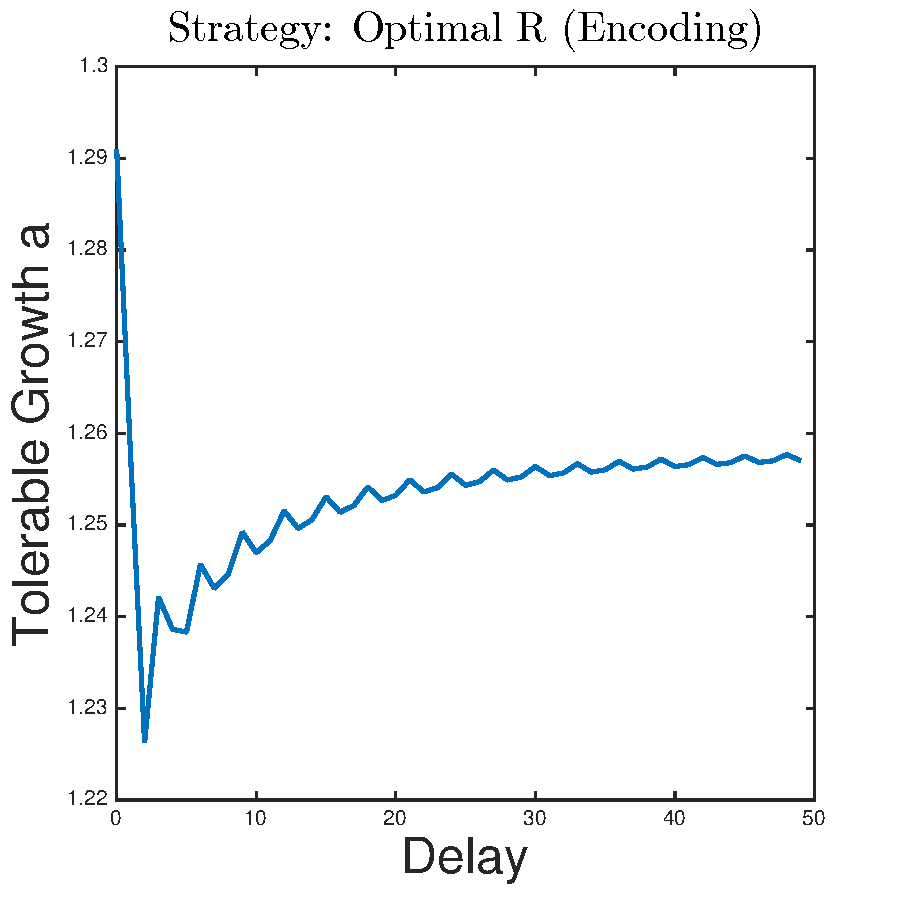
\includegraphics[width=0.3\textwidth]{150430_Dvsa}
  \end{center}
  \vspace{-20pt}
\end{wrapfigure}

%\begin{minipage}{0.5\textwidth}
%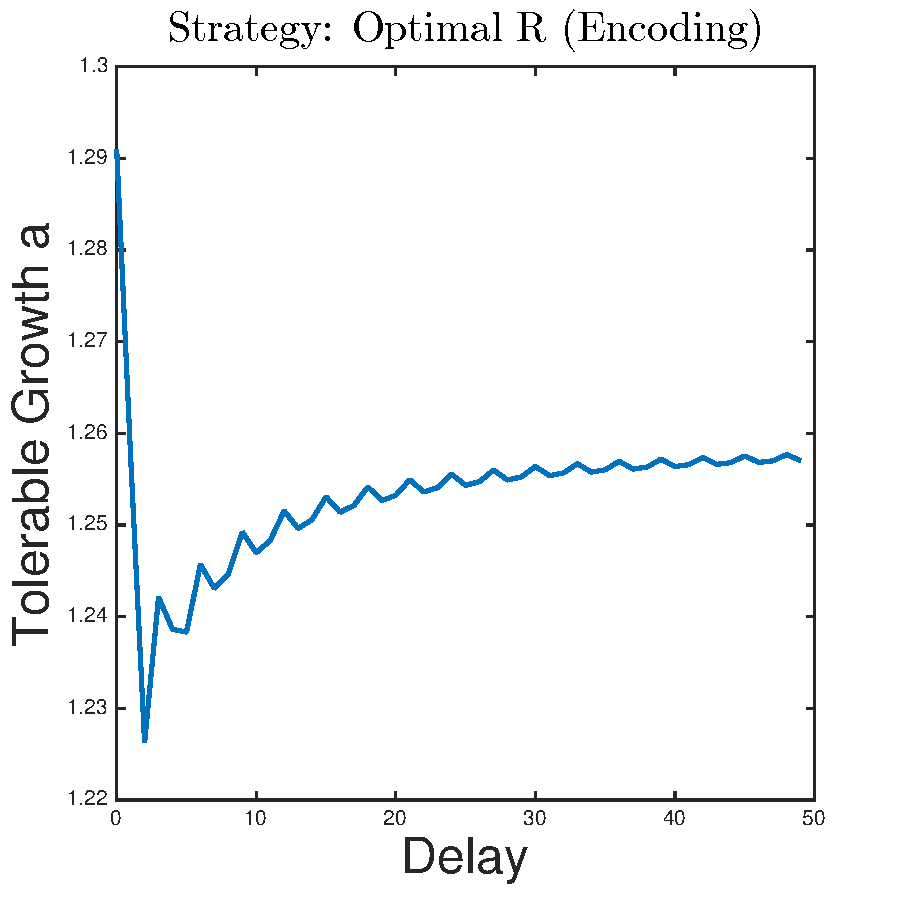
\includegraphics[width=\textwidth]{150430_Dvsa}
%\end{minipage}
%\begin{minipage}{0.5\textwidth}
This figure encapsulates our preliminary results on the delay tradeoff. In this figure, $R$ (the encoding rate of the observation) is chosen optimally based on the (D+1) length of the codeword. The Y-axis is the maximum growth the system can tolerate while remaining stable. Instantaneous control gives the best results, but may not be an option for real-world applications. Constrained by at least one unit of delay, a system performs better \textit{maximizing} delay. At the same time, the performance of the system improves asymptotically, meaning we don't need to achieve infinite delay to reap all possible benefits. The jaggedness of the plot stems from the discrete nature of the packet drop model. The encoder attempts to reach the optimal value for $R$, but is constrained by the number of packets it can allocate to information vs. redundancy.\\

Another interesting result is that the optimal encoding rate $R$ asymptotically decreases as delay increases. For small values of Delay (D = 1 or 2), $R$ is $\approx 0.65$. For example, if my codeword is length 3 bits, my encoder will allocate 2 bits to information and 1 bit to redundancy. For larger values of Delay ($D > 20$) the number decreases and converges to 0.34. For example, if my codeword is length 30 bits, my encoder will allocate 10 bits to information and 20 bits to redundancy. This comes from the interaction between quantization noise and message decoding, and is something we are still exploring.
\vspace{-10pt}
%\end{minipage}

%In addition, delay is closely tied to quantization noise and packet drop probability, but I'm only beginning to understand the interaction and relationship between these parameters. Delay is directly connected to information/number of bits available to the controller and \textcolor{red}{encoding strategies that should be employed.}

\subsection*{Future Work}
I have worked for the past year with Dr. Gireeja Ranade on this topic, but there is still much work to be done. There are two types of delay to be explored: "buffering" delay, where an observation is received every $D$ timesteps, and "streaming" delay, where an observation is received every timestep but is old (from $D$ timesteps ago). In addition, there are three different channels where delay could be present: $X \to Y, Y \to U, \text{ and } U \to X$. I have begun to understand different control strategies for working with these types of delay, but I have restricted myself to linear memoryless strategies. My future work will explore nonlinear or memory-based control strategies as a more optimal solution to the delay problem. I consider this the `control strategy' segment of my work, and it builds off of previous work from Ranade et al.\footnote{Gireeja Ranade and Anant Sahai. Non-Coherence in Estimation and Control. Allerton 2013.} and Schenato et al.\footnotemark[1]. In addition, I am curious to understand the `finite blocklength' effects described by Polyanskiy et al.\footnote{Yury Polyanskiy, H. Vincent Poor, and Sergio Verdu. Channel Coding Rate in the Finite Blocklength Regime. IEEE Transactions on Information Theory, Vol. 56 No. 5 May 2010.} In the future, I need to bring together these two parts, to characterize the delay tradeoff in a system.

\[ X(n+1) = a(X(n) - U(n)) + W(n) \]
\[ Y(n) = \left\{
     \begin{array}{ll}
       Q(X(n)) + V(n) & : n \equiv 0 \text{ (mod D + 1)}\\
       0 & : \text{else}
     \end{array}
   \right. \]
\[ Q(X(n)) = C(n)X(n) \]
\[ U(n) = \left\{
     \begin{array}{ll}
       L[X(n) \; | \; Y(n-D)] & : n \equiv 0 \text{ (mod  D + 1)}\\
       0 & : \text{else}
     \end{array}
   \right. \]
\newpage
\twocolumn   
   
\[ X(0) \sim N(0,1) \]
\[ W(n) \sim N \left( 0, \sigma^2_w \right) \]
\[ V(n) \sim N \left( 0, \sigma^2_v \right) \]
\[ m = D + 1 \]
\[ C(n) \sim N \left( 1, 2^{-2Rm} \right) \]
\[ \text{(Success) } \gamma  = 1 - 2^{-((1-R)m + 1)} \]
\[ \text{Packet drop } \sim \text{Ber} \left( \frac{1}{2} \right) \]

%I want to generalize beyond encoding with a Reed-Solomon scheme. 
\end{document}